
%% LyX 2.0.3 created this file.  For more info, see http://www.lyx.org/.
%% Do not edit unless you really know what you are doing.
\documentclass[english, a4paper,11pt]{article}
\usepackage[T1]{fontenc}
\usepackage[latin9]{inputenc}
\usepackage{setspace}
\usepackage{geometry}
\geometry{verbose,tmargin=2.5cm,bmargin=2.5cm,lmargin=3cm,rmargin=3cm}
\setlength{\parskip}{\bigskipamount}
\doublespacing
\setlength{\parindent}{0pt}
\usepackage{float}
\usepackage[sort]{natbib}
\usepackage{rotating}
\usepackage{graphicx}
%\addtolength{\oddsidemargin}{-.875in}
%	\addtolength{\evensidemargin}{-.875in}
%	\addtolength{\textwidth}{1.75in}

%	\addtolength{\topmargin}{-.875in}
%	\addtolength{\textheight}{1.75in}
\makeatletter
%%%%%%%%%%%%%%%%%%%%%%%%%%%%%% User specified LaTeX commands.
                           
                                       
\usepackage{array}                                          
\usepackage{longtable}                                       
\usepackage{calc}                                            
\usepackage{multirow}                                         
\usepackage{hhline}                                          
\usepackage{ifthen}                                           
%%  optionally (for landscape tables embedded in another document): 
 \usepackage{lscape} 
\def\inputGnumericTable{}  
\def\citeapos#1{\citeauthor{#1}'s (\citeyear{#1})}
\makeatother

\usepackage{babel}

\begin{document}
 
   
\title{Noise Traders or Smart Money? Evidence on Large Participant Behaviour in the Foreign Exchange Futures Market}
\author{Terence O Malley \\ 12254448  \\\\ Supervisor: Prof Morgan Kelly}
\maketitle

\begin{abstract}
The exchange rate disconnect puzzle remains one of the great shortcomings of international finance. One potential resolution of this puzzle is that investor heterogeneity is responsible for exchange rate volatility in the short-run. In this thesis I empirically assess a smart money- noise trader model of the exchange rate market by applying various multivariate statistical methodologies; from standard vector autoregression to the more recent method of vine copula inference.  Using data on futures market positions of various categories of investors, I show that there are marked differences in investor behaviour and that certain categories are positively correlated with futures contract prices. Whether this positive correlation is due to feedback trading or the better information/ market power hypothesis is unclear, though the evidence is balanced in favour of the former. 
 \end{abstract}
\clearpage

\section{Introduction}


\begin{quotation}
``It's because somebody knows something about it that we can't talk about physics. It's the things that nobody knows anything about that we can discuss. We can talk about the weather; we can talk about social problems; we can talk about psychology; we can talk about international finance ... ''
\citep{feynman2010surely}
\end{quotation}


\cite{friedman1953essays} postulated that, under a floating system of exchange rates, rational speculation by investors would bring exchange rates in line with their fundamental values. The experiences of the advanced economies post-Bretton Woods have largely rendered that prediction questionable however; volatility of exchange rates has increased compared with that of macroeconomic fundamentals \citep{floodrose}. 

Today, the market for foreign exchange claims the distinction of being the largest financial market in the world\footnote{with an average daily turnover of $\$ 4$ trillion! \citep{BIS2010}}. One might think it a reasonable position to believe such a market would be a liquid and therefore efficient market. Since the seminal piece by \cite{meese1983empirical} however, a growing body of work has shown that exchange rates are poorly described by any modern open economy macroeconomic model, and flutuate wildly and inexplicably when compared with fundamentals. This anomaly in international finance has come to be known as the {\it exchange rate disconnect puzzle}, lucidly defined by \cite{sixpuzzles} as the: \begin{quote} exceedingly weak relationship between the exchange rate and virtually any macroeconomic aggregates.\end{quote}

Various resolutions for the puzzle have been put forward to explain this apparent macroeconomic aberration. In their `anomalies' series, \cite{anomalies} note that: \begin{quote}
evidence suggests that explanations which allow for the possibility of market inefficiency should be seriously investigated.
\end{quote} One such method in solving the puzzle, which has enjoyed success, is the market microstructure approach{\footnote{See the work of \cite{evanslyons} who present evidence that exchange rate volatility is correlated with order flow. For a theoretical view see: \cite{bacchetta2006can}.}. 

Much of the development of the market microstructure discipline started with the noise trader model of \cite{kyle1985}. The basic idea behind a smart money- noise trader model is that traders in financial assets display heterogeneous behaviour: some branch of traders are well informed about the asset and trade based on expected utility maximisation, while others trade on information with no regard to fundamentals\footnote{For example, consider the contrasting utility maximisation problems of speculators and corporate treasuries, both of whom are likely to participate in the same market for foreign exchange}.

Other smart money- noise trader models of note are those of \cite{delongetala} and \cite{delongetalb}. In the former, noise traders are able to affect asset prices due to arbitrage- limiting risk aversion of smart money. In the latter, smart money are aware of the behaviour of noise traders and, by seeking to profit off positive feedback trading, they amplifying the noise and move prices further away from fundamentals. Indeed \cite{frankelfroot} show evidence from survey data of the prevalence of extrapolative expectations among foreign exchange traders. 

The prediction of these models is that there exist discernible differences in how different groups of traders behave in the market. Though work has been done in applying this theory to a foreign exchange market setting \citep{jeannerose, bacchetta2006can}, an extensive empirical literature analysing market participant data is not as prevalent\footnote{One can imagine why market participants may be loathe to voluntarily release information about their market positions.}\footnote{\cite{kelly1997noise} tests a smart money-noise trader model in the context of the stock market and finds evidence that data behave as predicted by the model.}. 

For the investor heterogeneity approach to help resolve the exchange rate disconnect puzzle, its predictions must match that which is observed in the marketplace. The contribution of this thesis will be to offer support to or contradict the investor heterogeneity conjecture by means of an empirically evaluation of a smart money-noise trader model in the foreign exchange market. The two papers closest in spirit to this thesis are those by \cite{wei1997big} and \cite{corsetti2002role}. Both papers use the same data set from different periods and find opposing evidence in support of a smart money- noise trader view of currency markets. 


\section{Literature Review}

\cite{wei1997big} study private information in currency markets using data from the US Treasury on foreign exchange positions taken by large traders. They too are interested in gathering empirical evidence about ``asymmetric information among traders that may be price relevant''. As the authors point out, any evidence that is favourable to an investor heterogeneity model may indicate why existing models of international macroeconomics explain exchange rates so poorly; the consequence being that model- builders should seek to integrate models from market microstructure into open economy macroeconomics. Those authors' data set consists of aggregated data on foreign exchange positions of large participants in spot and derivative markets. The data are weekly observations from a relatively short time- series: from January 1994 to December 1996. 

The data set employed in this study has both a strength and a weakness. The strength is that the data set contains information from both spot and derivative markets. It is likely that any study concentrated on any one of these markets in isolation may be missing vital information on the `bigger picture' of currency holdings positions of traders\footnote{Indeed in 2010 the BIS reported that foreign exchange swaps accounted for more of the global fx market than spot transactions did.}.  Secondly, the weakness is that large investors are treated as a homogeneous category. Given that the hypothesis under investigation concerns investor heterogeneity, it seems possible that the different investors making up the `large trader' classification in their study may not consist of a uniform trader type, but rather of several classes of investors acting disparately. 

The authors findings are perhaps surprising. Using a simple linear regression model of returns and net foreign exchange positions, they report that \begin{quote}position taking by large participants does not help to forecast subsequent appreciation of the exchange rate.\end{quote}

\cite{corsetti2002role} study the same data as the previous authors, though they do so several years after and with the benefit a larger time-series. Interestingly they report evidence to the contrary. They find, using a linear regression model where the exchange rate level is the dependent variable, that the coefficient on net positions is positive. They conclude that either large traders do have either better information  (better information hypothesis) or can directly influence exchange rate levels through sheer size of their positions alone (market power hypothesis). They do not find substantial evidence however that foreign exchange returns are strongly correlated with net positions, which they attribute to the possibility that such high-frequency returns exhibit a high degree of noise not present in the lower-frequency movements of exchange rate levels. 


\section{Data}

The objective of this thesis is to empirically assess a smart money- noise trader model in the foreign exchange market. In order to test the smart money- noise trader hypothesis, data are needed on positions taken by different groups of traders in the asset in question. Unfortunately most foreign exchange trading occurs over-the-counter and is not transacted through a clearing house; the result being that data on traders' positions are either not collected or are proprietary in nature. There are some data available such as that collected by various central banks in major currency trading locations (NYC, London etc) and also the triennial BIS survey of foreign exchange trading activity. This data consist of mostly sparse, short time series and are therefore not suited to an extensive and legitimate econometric analysis. 

Fortunately for this author however, there is a large market in foreign exchange futures contracts, which are traded on the Chicago Mercantile Exchange and therefore are subject to regulation by the Commodity Futures Trading Commission (CFTC). As part of its mandate the CFTC collects confidential daily data on positions taking by large traders in various futures markets- including foreign exchange. The data are released weekly under the `Traders in Financial Futures (TFF)'. In late 2010 the CFTC released four years of historical data reclassified into the TFF format (i.e. positions data disaggregated by large trader types). This data, along with the data collected since then, plus futures price data, form the basis of this thesis. 

The TFF report contains information on open interest of large traders in large futures markets and separates large traders into four categories (one sell-side and three buy-side): dealer/ intermediary (sell-side), asset manager/ institutional, leveraged funds and other reportables (buy-side). It is important to note that the sell- and buy-side distinctions may not necessarily correlate to each group's actual behaviour in financial markets, but rather they designate general functions across markets. For example, leveraged funds (buy-side) may take short-positions in futures contracts and dealers (sell-side) may be long this same contract. Table 2 describes the classification of each participant. 



\begin{table}[ht]
\begin{tiny}
 \input{tables/participant}  
\addtocounter{table}{-1}
\caption{Futures Market Participant Classification}
\end{tiny}
\end{table}  

The report lists two variables that are of interest to this thesis for each participant. The first is short positions in futures contracts, and the second is long positions. 

The second piece of data collected are prices of futures contracts. This data is easily attainable from Thomson-Reuters EcoWin Pro, which is open for access to University students. 

The extent to which this data can answer my answer my research question is interesting. As was highlighted in the previous section in my discussion of \cite{wei1997big}, the global foreign exchange market is spread across both spot and several derivative markets. It is therefore probable that data from the futures market alone will not tell the whole story. I take two views on the matter: either the futures market can act as a noisy proxy for the overall market (with the accompanying loss of statistical power) or as is my preferred approach - treat this analysis as purely a study of the futures market. Though a study of the former may apply more generally, it is essentially a case of data trade-off: either study total foreign exchange positions for an aggregated large trader category or study one isolated market with data disaggregated by large trader type. For this thesis I choose the latter.  

\subsection{Data Set Properties}
The data set that will be studied in this thesis is a combination of the Thomson-Reuters price data and TFF positions data. The TFF data (long and short positions for each participant) are a weekly time series that run from the 13th June 2006 to the 31st December 2012. Futures market data on six major currencies are chosen for analysis. They are: Australian Dollar (AUD), Canadian Dollar (CAD), Swiss Franc (CHF), Euro (EUR), British Pound (GBP) and Japanese Yen (JPY). 

The price data (expressed as the cost of one unit of currency in US dollars i.e as an exchange rate\footnote{Price for JPY given in cost in USD of one million units of yen.}) for a futures contracts in each currency are downloaded at weekly intervals to match the positions time series and the two data sets are merged. To form the final data set on which the econometric analysis is carried out, variables for the net positions for each large participant are created by netting long and short positions of each participant type. At this point another variable is created; a net variable that is an aggregate of all large trader positions in each market.  These net variables, along with the price data, for each of the six currencies constitute the final data set. A description of the data set is given below. 


\begin{table}[ht]
\begin{tiny}
 \input{tables/descip}  
\addtocounter{table}{-1}
\caption{Description of data set}
\end{tiny}
\end{table}

\subsection{Summary Statistics}

Summary statistics for the data set are presented in table 3. The time series is made up of 343 weekly observations. It is clear from the sample skewness and kurtosis that the data for the various processes are not normally distributed. This will have implications for correlation analysis later on; so is noted at this point. The difference between the scales of the price and position data is also noted. 

\begin{table}
\begin{tiny}
 \input{tables/summ}  
\addtocounter{table}{-1}
\caption{Summary Statistics}
\end{tiny}
\end{table}

\subsection{Pairwise Combinations}


In total there are eight variables in the data set, one of which is the time index and a second which is the currency factor. This leaves six variables containing the data of interest: price and the net position variables. The hypotheses of interest in this thesis can be broken into two sets. Firstly what is the relationship between price and the various net positions of large traders? Secondly what is the interrelationship between the net positions of the large traders? Essentially the analysis will deal with taking different pairwise combinations of the data for each currency and assessing correlation between them. In order to do this, a simple combinatorial algorithm can be used to yield the following matrix of unique pairwise combinations\footnote{The R statistical environment \citep{rstats} is used for the analysis in this paper in its entirety.}. 

\begin{table}[H]
\begin{tiny}
 \input{tables/pairs}  
\addtocounter{table}{-1}
\caption{Pairwise Combinations}
\end{tiny}
\end{table}

The actual results from the algorithm produce 15 results. However I am not interested in the combinations of $net$ and its constituent series, so these 4 results are removed. 

\clearpage
\subsection{Visualisation}

As a first step in answering my research question, I visualise different aspects of the data set to guide analysis. Firstly I plot a multivariate time series graph\footnote{This method of visualising multivariate time series data is provided by \cite{mvtsplot}.} for the currencies to answer a relatively simple question: Are large traders a homogeneous group in their position-taking? This question is motivated by the \cite{wei1997big} paper, in which those authors use data that do not differentiate between large traders, but rather treats them as one uniform group. The plot for the Australian dollar data is displayed in figure 1. 

\begin{figure}[h]
\begin{center}
\includegraphics[scale=0.8]{heterogeneity}
\end{center}
\caption{Trader Heterogeneity in the Australian Dollar Futures Market. The large centre pane shows the  net positions  time series, each row is one the margins of this series; $other\_net$, $asset\_net$, $lev\_net$, $dealer\_net$. The series is smoothed using a global spline and represented on a colour scale from purple to green, deep purple being the minimum (a large short position) and deep green being the maximum (a large long position). The panel on the right shows the distributions of the margins and the bottom pane shows the entire smoothed series (which corresponds to the $net$ variable in the data set).}
\end{figure}

The reader can see the limitations of the aforementioned study from this simple graphic. There are clear differences in how each of the large trader types behave in the market. Noticeable is the tendency for leveraged funds and dealers to take the extreme opposite positions as one another. Indeed the relationship seems to be near perfectly negative. Other reportables and asset managers do not take quite as extreme positions (the summary statistics also show large differences in standard deviations between the groups' positions) and do not seem to be as correlated with the other participants. 

The properties of the time series are also of interest, so as an informal first step to explore the possibility that the series are integrated, I plot each below\footnote{The lattice graphics package is attributable to \cite{lattice}}.

\begin{figure}[ht] 
\begin{center}
\includegraphics[scale=0.8]{priceviz}
\end{center}
\caption{Time series for price data}
\end{figure}

As one might expect - and in the spirit of the random-walk hypothesis of asset prices - the price series all seem to feature a stochastic trend. 

\begin{figure}[ht]  
\begin{center}
\includegraphics[scale=0.8]{positionsviz}
\end{center}
\caption{Time series for positions data. Note that all series have been scaled by division of one standard deviation for visualisation. For an idea of relevant magnitudes, please see summary statistics.}
\end{figure}

The positions series in figure 3 look more like stationary process on first inspection, though there are noticeable outliers in the $other\_net$ (red) and $asset\_net$ (orange) series. Next I move onto formal tests to assess the stochastic properties of the data. 


\subsection{Unit Root Testing}

I begin by running Dickey-Fuller regressions on every process in the data and calculating the Dickey-Fuller test statistic \citep{dickey1979}. Results from this test and also from the augmented specification are presented in table 5\footnote{D-F test statistics are reported here to save space in the main body of the text. The first statistic is the standard Dickey-Fuller statistic and the second from a regression augmented with six lags: $k = (n-1)^{1/3}$.The full regression results are included in the appendix.}.

\begin{table}[H]
\begin{tiny}
 \input{tables_new/ADF}  
\addtocounter{table}{-1}
\caption{(Augmented) Dickey-Fuller Test Statistics.}
\end{tiny}
\end{table}

As expected, the null hypothesis cannot be rejected for the price series. There is evidence that the net series are stationary: the null is rejected in most specifications across currencies at the 5\% significance level. At higher lags the null is rejected at the 10\% level except for the  Euro and pound. The same roughly applies to the dealer series. Most specifications reject at 10\%. Again the augmented statistic is not rejected for CAD, EUR and GBP. The asset series is more problematic, the null is not rejected for AUD, GBP and JPY. From figure 3 though, it is noticeable that there is a possible structural break in the AUD asset\_net series in late 2011. There also seem to be large outliers in the GBP series and a possible structural break in late 2011 in the JPY series. These factors may weaken the power of the tests to reject the null. The tests mostly reject for the lev\_net series also. The augmented specifications do not reject for CAD and EUR. The tests reject for the other\_net series in all specifications except for the augmented regression for GBP.  

It is known that the Dickey-Fuller test can suffer from a lack of power to reject the null hypothesis of a unit root \citep{kpss}. As a second test: the \cite {pptest} test\footnote{Available in the R package `tseries' \citep{tseries}}, is performed on the same data for robustness. Again the null hypothesis here is that the series contains a unit root. The tests fail to reject the null for the price series. The tests do reject the null for most of the positions data however. The exceptions are the net series for EUR, the dealer series for CAD/EUR/GBP, leveraged fund positions for GBP/JPY and the other series for GBP.  

\begin{table}[H]
\begin{tiny}
 \input{tables_new/pptest}  
\addtocounter{table}{-1}
\caption{Phillips-Perron Test Statistics}
\end{tiny}
\end{table}

To conclude this section, the price series do seem to follow a random walk and the positions data show more properties of stationarity. There are notable exceptions to the latter however, and this is kept in mind as a caveat when assessing correlation in the next section. 


\section{Correlation and Dependence Modelling}

\subsection{Scatter Plots}

As a first attempt at understanding any relationships between the variables, scatter plots for every pairwise combination are produced, along with fitted lines. Figure 4 shows a visualisation of the relationships between price and the positions data. Figure 5 shows the relationships between the different positions variables. 

From figure 4 it is noticeable that the fitted line is not always an accurate representation of the data. The results are nonetheless striking. A simple linear relationship shows a negative relationship between net positions of all large traders and price. This result is perhaps surprising, though it would be too eager to draw inference from a simple linear representation. The exception is the yen, where a simple linear function seems to fit the data reasonably well and is in fact positive. For dealer positions the picture is a little clearer. Again a linear model does not fit the data too well, but the relationship is consistent across currencies. Dealer positions seem to be negatively correlated to prices: a surprising results perhaps. A reasonable prior might be that dealers, if any party, might be the most likely to represent smart money in the market due to privileged access to customer order flow. The picture for leveraged fund positions is the opposite. A linear model seems to fit reasonably well and shows a positive relationship between leveraged fund positions and price. Maybe leveraged funds are the smart money in the market. 
The results from asset manager and other reportable positions are less consistent than the previous two. For asset managers a linear model shows a negative relationship for the Australian dollar, positive for the yen and none for the rest. For other reportables the estimated relationship is largely negative, except for GBP where the line of best fit does not seem to represent a good fit in the slightest. At this early stage a picture of the data is forming: leveraged funds are smart money, other reportables are noise traders, asset managers are inconclusive and dealers are also noise traders. This picture of dealers as noise traders does not seem to make sense to this author, and remembering the nature of a dealer's role in the market, it may make sense that dealers are on the wrong side of price movements in one market, while hedging in another. 


\begin{figure}[h]  
\begin{center}
\includegraphics[scale=0.775]{scatter1}
\end{center}
\caption{Scatter plots with fitted lines: price and positions}
\end{figure}
%% optional code for 2 col smaller plot
%> pdf('scatter1.pdf', h=5,w=9)
%> grid.arrange(p1, p2, p3, p4, p5, ncol = 2)
%> dev.off()

The scatter plots in figure 5 show the relationships between the various parties in the futures market. The two rows that stick out are rows 2 and 5. The relationship between leveraged funds and dealers is nearly wholly explained by a simple negative linear relationship. This result was hinted at by the multivariate time series plot of the Australian dollar, and may offer an explanation as to why dealer positions seem to be negatively correlated with prices. It seems that dealers and leveraged funds take the extreme opposite positions to each other. Remembering what was seen in the previous plot, it is tempting to conclude that leveraged funds represent smart money and dealers are not noise traders, but merely facilitate leveraged funds positions in the market. There also appears to be a consistent positive relationship between leveraged fund and asset manager positions, though the relationship is a lot noisier than that between funds and dealers. 


\begin{figure}  [h]
\begin{center}
\includegraphics[scale=0.775]{scatter2}
\end{center}
\caption{Scatter plots with fitted lines: positions}
\end{figure}

\clearpage

\subsection{Measures of Correlation}

I now perform relatively simple formal measures of correlations and tests of hypotheses to judge how reliable inference from the simple scatter plot is. I utilise three procedures in this section. The first is the simplest measure of correlation: Pearson's $k$. I then estimate a non-parametric measure: Spearman's $\rho$. Finally I augment the estimates of Pearson's $k$ by running a least squares regression with robust standard errors and obtain sample estimates of the coefficients of interest. 

Firstly the results from the estimates of $k$ are reported in table 7. The results are quite interesting in that the estimates seem to be consistent across currencies and largely statistically significant. Perhaps surprisingly - given the results of \cite{corsetti2002role} - the correlation between net positions and price is negative. When the positions data are disaggregated into groups, a clearer picture emerges. The large negative relationship between price and dealer positions is statistically significant, as are most of the estimates for price and other reportable positions (GBP is the exception). The estimates of correlation between price and leveraged fund positions do show a positive relationship; they are again consistently significant. Correlation between asset manager positions and the level of price is not as clear: it is negative for AUD and positive for CAD, CHF, GBP and JPY (the magnitude is generally lower than that of leveraged fund positions), and not significant for EUR. On the question of interrelationships between large trader positions, the tests report significant and large estimates for the dealer/leveraged fund relationship, significant positive estimates for asset manager/ leveraged fund positions, significant negative estimates for asset manager/ dealer positions. The relationship between other reportable and dealer positions is largely inconclusive though there are some significant results. The estimates for other reportables and leveraged fund/ asset managers is largely negative and statistically significant. 


Though Pearson's $k$ is a simple way of estimating the relationships between the variables, there are many reasons to doubt the validity of the estimates. Firstly - as was evidenced in the summary statistics- the data are highly non-normal, thus violating the normality of data assumption required by this measure. Secondly, the price series contain a unit root and so any estimate of $k$ from this sample will not converge to the true correlation but diverge as the sample size increases. A third problem is that $k$ only describes linear relationships, yet as seen previously in the scatter plot, the relationships can rarely be defined as linear. For this final reason, Spearman's $\rho$ is also estimated. This non-parametric estimator is not restricted to estimating linear relationships, though it does require any relationship to be monotonic - a much more feasible assumption for this data. Results are presented in table 8. They are evidently very similar in magnitude and statistical significance to the results from table 7. 

Finally an OLS regression is performed. In most specifications, the differing scales of dependant variables and regressors will lead to low estimates of coefficients. To obtain a sensible estimate of the relationships, two methods are used. For the first, I estimate a standard linear regression model and scale coefficients upwards as in the study of \cite{corsetti2002role}. The second method involves scaling all variables by dividing by their standard deviations. In this method the coefficient of the regressor is identical to Pearson's $k$. To correct for autocorrelation in the residuals (Durbin-Watson tests reject the null hypothesis of no autocorrelation of residuals in all specification), robust standard errors are obtained using the method of \cite{vcovHAC} and p-values calculated. 

Results of specifications where price is the dependent variable are presented in table 9. Again the results for net positions of all large traders here are wholly different to those reported from the same linear model in \cite{corsetti2002role}: the sign has changed. The regression of price on leveraged fund positions is similar to their results however. Results for standardized regression only on the positions specifications are reported in table 10. Both results are similar to those for estimates of $k$; though with corrections for autocorrelated residuals many estimates are no longer statistically significant.  

\begin{table}[ht]
\begin{tiny}
 \input{tables/pearson}  
\addtocounter{table}{-1}
\caption{Estimates of Pearson's $k$}
\end{tiny}
\end{table}

\begin{table}[ht]
\begin{tiny}
 \input{tables/spearman}  
\addtocounter{table}{-1}
\caption{Estimates of Spearman's $\rho$} 
\end{tiny}
\end{table}

\begin{table}[ht]
\begin{tiny}
 \input{tables_new/ols_new}  
\addtocounter{table}{-1}
\caption{OLS regression of price and position variables }
\end{tiny}
\end{table}

\begin{table}[ht]
\begin{tiny}
 \input{tables/olspositions}  
\addtocounter{table}{-1}
\caption{OLS regression of position variables}
\end{tiny}
\end{table}

\clearpage

\subsection{Dependence Modelling Using Vine Copulas}

A better to way to model the dependence within the processes in the data is to use copula methods. As mentioned previously, Pearson's correlation relies on the assumption that the data is normally jointly distributed. This is not the case for most financial data; indeed summary statistics showed that this data set is no exception. Copula functions were first described by \cite{Sklar} as a way of measuring dependence between random variables. Sklar's theorem states that a joint distribution function $F(x)$ can be separated into its univariate marginal uniform distribution functions and a copula function that describes the relationship between them. For a vector of random variables, $x = [x_1, x_2]'$: 

$$F(x) =  C(F(x_1), F(x_2))$$ where $C()$ is a copula function describing the dependence between the uniformly distributed margins. 

There is a rich set of Copula functions to choose from to describe the dependence structure between two marginal distributions, and so this method of determining dependence makes more sense for irregular data such as that used in this thesis. 

A recent advance in high-dimensional copula modelling is that of vine copula methods. Vine copulas allow the modeller to specify a `tree'-like structure within the data and estimate a different copula for each pairwise combination in that tree. This method is perfect for the multivariate data in this thesis (i.e. many variables whose interdependence is of interest). For example a Gaussian copula can be specified for the relationship between price and leveraged fund positions, and a completely different copula ,e.g. Gumbel copula, can be used to model the relationship between leveraged fund and dealer positions. Fortunately this method has recently been implemented as the package $CDVine$ in R by \cite{brechmann2012modeling}. In this section I will follow the methodology of those authors, illustrating with the Australian dollar as an example and then providing empirical estimates of a fourth measure of correlation - Kendall's $\tau$ - based on the estimated vine copula parameters. 

Firstly the data set must be transformed to `copula data' i.e. the data must lie on the unit interval. This is achieved by non-parametrically transforming the data using each variables' empirical cumulative distribution function (See figure 6).

\begin{figure} [ht] 
\includegraphics[scale = 0.65]{ecdf}

\caption{Transformation to copula data. The data in the margins of a pair copula must lie on the interval [0,1]. This transformation is achieved by estimating the CDF (middle panel) and applying this function to the data. This transformation is shown in the third panel. After the transformation, values of $1$ are replaced with $1 - 10^{-10}$ to avoid computational issues. }
\end{figure}

\begin{figure} [ht] 
\begin{center}
\includegraphics[scale=0.8]{contour}
\end{center}
\caption{Contour plot. Above the diagonal are scatter plots of the transformed data. Below are the empirical contour plots. Evidence of dependence is evident between price and asset \& lev\_net. Interdependence among participants is also evident.}
\end{figure}

To assess the dependence structure within the data a C-vine Copula is estimated. This is achieved by specifying a tree structure between pairwise combinations of the data and estimating a different copula for the margins of all these pairs. The structure of the tree is reported in table 12. This structure was chosen manually to fit the structure of the research question i.e. what is price's relationship with participants and what is the relationship between the participants? The first tree therefore assesses the former relationship and the rest explore the latter. Also note that the $net$ variable is not included in the tree, as it is a composite of the individual positions data and so it would not make sense to include it. 

\begin{table}[ht]
\begin{tiny}
 \input{tables/cvine} 
 \end{tiny}
\addtocounter{table}{-1}
\caption{C-Vine Structure}
\end{table}

Two C-vine models are estimated by maximum likelihood methods using different pairwise copula families and compared via values of the log-likelihood. The first family of copulas is estimated directly using the CDVine package, which chooses each copula family for the first tree and then proceeds to the next trees one-by-one and estimates the copula based on the conditional pairs along the way. The second family of copulas used is just a simple Gaussian copula for every (conditional) pair. 

\begin{table}[ht]
\begin{tiny}
 \input{tables/select}  
\addtocounter{table}{-1}
\end{tiny}
\caption{Copula Selection}
\end{table}

On the basis of the higher log-likelihood, the first model is chosen and is estimated by joint MLE. The empirical values of Kendall's $\tau$ can then be computed based on a transformation of the copula parameters. To apply this methodology across the six currencies I write an algorithm to estimate the c-vine copula structure, compute the parameters by joint ML and then compute $\hat{\tau}$. The results from this procedure are printed in table 15, and a graphic representation of the C-vine tree is presented in figure 8. 
\clearpage

\begin{table}[ht]
\begin{tiny}
 \input{tables_new/tau}  
\addtocounter{table}{-1}
\caption{Joint ML empirical estimates of Kendall's $\tau$ based on computed c-vine structure. Please refer to table 11 for a description of the structure.}
\end{tiny}
\end{table}
 

The results confirm what was evidenced by the previous measures of correlation. The relationship between price and dealer positions is negative; between price and leveraged fund positions it is positive and there is weaker evidence for the other two types of large trader. Between participants, there is again a large negative relationship between dealers and leveraged funds, and a slightly less negative relationship between dealers and asset managers. The estimated relationship between asset managers and leveraged funds is negative here interestingly, as is the estimated relationship between asset managers and other reportables.

\begin{figure}[ht]
\begin{center}
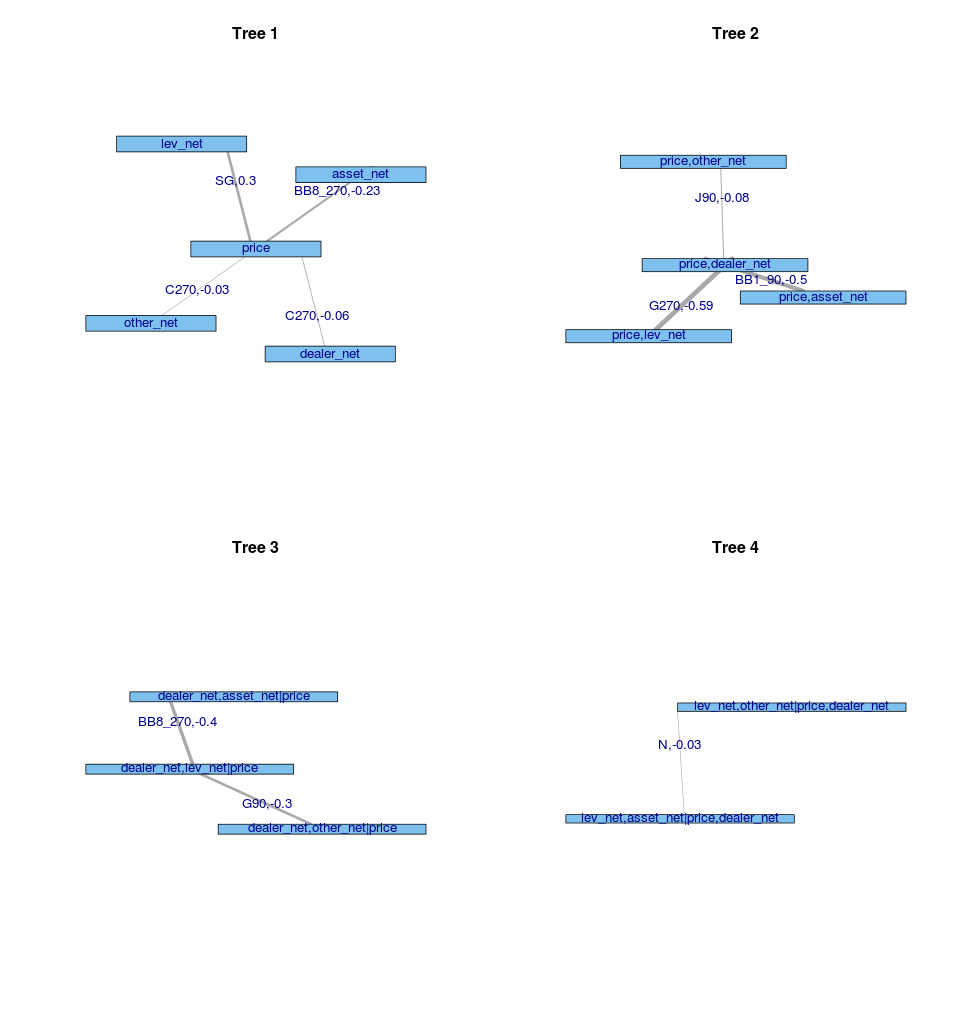
\includegraphics[scale = 0.4]{tree.png}
\end{center}
\caption{C-vine tree. Pair-copula families and values of Kendall's $\tau$ are reported. The width of each branch is calculated using $\hat{\tau}^{MLE}$. N = Normal (Gaussian) copula, G = Gumbel copula, SG = Survival Gumbel copula (Gumbel rotated $180^{\circ}$), C = Clayton copula and BB8 = BB8 copula. A number after the copula label describes a rotation of a copula e.g C270= Clayton copula rotated $270^{\circ}$.}
\end{figure}


\clearpage
\section{Multivariate Time Series Methods}

The previous section dealt with some topics regarding the dependence structures within the data set. This section however deals with more specific time series methods. Noticeably lacking from the previous section was any mention of lags. It might be a reasonable position to take that many of the relationships I am interested in exploring in this thesis are dynamic and evolve differently over time: therefore the previous section - while helping to illuminate different aspects of the data - is not entirely suited to analysis of the data set. Another issue highlighted in section 3 was that of non-stationarity: the methods used in the previous section cannot be thought of as robust given the non-stationary of certain processes in the data. Differencing the data would have resolved this problem\footnote{Unit root tests on differenced data confirms.} but information would have been lost in the process \citep[p 301]{enders}.

To demonstrate the above, consider the plot in figure 9 of the empirical cross correlation functions for the Australian dollar. Here price has been first differenced to render it stationary. What is noticeable first is that for the differenced price series, there are no significant cross correlated lags at 0 i.e there is no statistically significant relationship between differenced price (i.e weekly returns) and the positions series at lag 0. However lagged correlations between price and positions are significant for net, lev\_net, other\_net and dealer\_net. There are none however for asset\_net. Already this simple plot gives an idea as to the dynamic properties of the data set; net and dealer positions are negatively correlated with price changes at negative lags, leveraged fund positions are positively correlated at negative lags, asset managers positions and price changes are not correlated and other reportable positions are negatively correlated at positive lags with price changes. Already a simple story of the differences in the dynamic behaviour of each group is revealed. Dealers and leveraged fund positions seem to come after price changes and other reportable position come before here. This is possible early evidence in support of \citeapos{frankelfroot} result on positive feedback trading in the foreign exchange market. 


To give a better answer to the research question, I wish to test the hypothesis that there is a dynamic relationship between some pairwise combinations of the variables.  I adopt the standard vector autoregression (VAR) framework to do so. 
\begin{figure}  [ht]
\begin{center}
\includegraphics[scale=0.5]{ccf}
\end{center}
\caption{Cross-Correlation Function for AUD. On the x-scale is the time lag between the two series}
\end{figure}

\subsection{Vector Autoregression}

To explore the idea that there may be dynamic linear interdependencies between different pairwise combinations in the data, I estimate a reduced-form vector autoregression (VAR) for each of them. As a result there are $6 \times 11$ VAR($k$)s to be estimated. To illustrate this approach, consider $Z_t = [z_1, z_2]'$, which is a matrix containing one of these 11 combinations for one of the 6 currencies. The vector $z_1$ can either take the form of a price variable or a positions variable. Vector $z_2$ here is always a position variable. The system I estimate for every pair, for every currency takes the form: 
$$ Z_t = B_0 + B_1\sum_{p = 1}^{k} Z_{t-k} + \epsilon_t$$ This system is fully identified by construction and the parameter matrices can be estimated by OLS.  Choosing the number of lags, $k$, for each of these VARs is a non-trivial task. The approach I have opted to use involves writing an algorithm sequentially combining functions from the `vars' package in R {\citep{vars}}. The algorithm chooses the 11 relationships of interest for each currency, performs two selection criteria: Akaike information criteria (AIC) and Schwarz- Bayesian information criteria (BIC), and then estimates a VAR($k$) where $k$ is pre-decided by the user as either: $$k\,=\,max\{k(AIC), k(BIC)\}$$ or $$k\,=\,min\{k(AIC), k(BIC)\}$$ The reason for this two-step approach (meaning $66 \times 2$ VARs) is to eliminate any possibility that a misspecified VAR is giving spurious results. For example AIC and BIC can often determine wholly different estimates of $k$, a large $k$ may result in spurious statistical significance (type I error) and a low $k$ may result in a type II error. 

\subsection{Granger- Causality Analysis}

Following this model selection, the algorithm then proceeds to test the hypothesis that the lags of one of the variables in the system does not help in explaining the other (standard Granger-causality test). The null hypothesis for this test is of no Granger-causality, which I might expect as a reasonable position consistent with an efficient market hypothesis view of futures contracts prices. A standard F-test is used to test these joint $k$ restrictions for each model. 

Results from these tests are presented in tables 14 and 15. Table 14 shows results from VARs estimated on the relationships between prices and participant positions. Table 15 shows results from estimates of relationships between market participants' positions. 

\subsubsection*{Price and Large Trader Positions}

\begin{table}[ht]
\begin{tiny}
 \input{tables_new/granger_price}  
\addtocounter{table}{-1}
\caption{Granger-causality tests: price and large trader positions}
\end{tiny}
\end{table}

Results from table 14 show tests of the null hypotheses of non-causality in both directions for the systems containing price as a vector. The first two columns show the maximum lag specification and the second two show the minimum lag specification. The purpose of these tests is to see whether there exists a causal relationship between price of futures contracts and position taken by large traders. Any evidence to support that relationship could be reconciled with a smart money- noise trader model i.e. some participants can take causally prior positions before movements in price levels or can directly move the market with positions. 

There is explicit evidence from both sets of models that price does help predict net positions of all large traders, net positions of dealers and leveraged funds. Indeed the tests reject universally across all currencies and for both lag specifications in that direction of Granger-causality. There is some evidence also that price Granger-causes asset manager positions, but the evidence is weaker and is not independent of lag selection (for which there is high variance). Perhaps the longer lag specifications are appropriate if asset managers are slower to react to price movements than leveraged funds and dealers - which is perhaps feasible. 

Going in the other direction of Granger-causality - from position to price - there is little to no evidence to reject the null of no causality. There is an exception for asset managers in JPY but this results is not robust to a smaller lag model specification. There is significant evidence however to reject the null for other reportable positions in the Canadian dollar. There is a strong rejection of the null for both models: a VAR(1) and a VAR(9). A look at the time series in section 3 shows a very large spike in other reportable positions at a time when the price for Canadian dollars fell. As this category contains central banks, it seems plausible that this rejection of the null is a reflection of Bank of Canada intervention (the magnitude of the spike is much larger than normally associated with other reportables positions) rather than prior-position taking by corporate treasuries. Preliminary results from this first model are not kind to the better information or market power of large trader hypotheses. Indeed it seems more likely that large traders are engaged in positive feedback trading. 



\begin{table}[ht]
\begin{tiny}
 \input{tables_new/granger_positions}  
\addtocounter{table}{-1}
\caption{Granger-causality tests: among large trader positions}
\end{tiny}
\end{table}
\clearpage

\subsubsection*{Among Large Trader Positions}
Table 15 shows results from Granger-causality test for VAR systems involving just traders' positions. A rejection of non-causality may provide evidence to support a positive- feedback style noise trader model of large trader behaviour. Again there are two specifications: maximum lag model and minimum lag model. 

Although there are exceptions, there is little evidence to suggest that different groups' positions are causally prior to another groups'. There are some significant results at a 5\% significance level, but they are hardly consistent across specifications and currencies. For example there is evidence that dealer positions are causally prior to asset manager positions in CAD, and are causally prior to leveraged fund positions in CHF and other reportables in EUR. There is also a rejection of the null of non-causality from the positions of leveraged funds to asset mangers in CAD, from other to asset managers in AUD and from leveraged funds to others in GBP. Indeed from these results, a positive-feedback noise trader story of large trader interrelationships does not seem consistent. 

\subsection{Lag Augmented Granger- Causality Analysis}

An issue that must be addressed in the preceding section regards the non-stationarity of the price data. The VARs are all estimated in levels to prevent loss of information from first differencing \cite[p.244]{lutkepohl2005new}. Unfortunately in this case, the asymptotic properties of the test statistic may not be valid under the null \citep{lutkepohl2005new, varsvignette}. Fortuitously however, both \cite{toda1995statistical} and \cite{lutkepohl1996} provide the methodology to test restrictions on a VAR estimated in levels, where some or all of the processes are integrated or cointegrated\footnote{See \cite{lutkepohl2005new} for a textbook treatment.}. To do so the optimal lags $k$ are determined as usual and a VAR with lags $m = k + d_{max}$ is estimated, where $d_{max}$ is the maximum order of integration of the processes in the system. To test restrictions such as the joint restrictions in a Granger-causality test, the usual restrictions can be applied to the first $k$ lagged coefficients and covariance matrices using a Wald test with $k$ degrees of freedom. The $\chi^{2}$ test statistic is then asymptotically distributed under the null.

I carry out this analysis for the price and position VAR systems and present the results in table 16\footnote{R package `dynlm' \citep{dynlm} is used to estimate the linear relationships and `aod' \citep{aod} is used to test the appropriate linear restrictions.}. The conclusions from the non-corrected tests largely remain: there is evidence that prices Granger-cause the positions of dealers and leveraged funds and weaker evidence that prices Granger-cause asset manager positions. Again there is little to no evidence of in favour of the reverse relationship: in fact the hypothesis is no longer rejected for CAD and other\_net, further evidence that one small period was responsible for this rejection. 


\begin{table}[ht]
\begin{tiny}
 \input{tables_new/typrice}  
\addtocounter{table}{-1}
\caption{Lag-augmented causality tests}
\end{tiny}
\end{table}

\subsection{Instantaneous Causality Analysis}

I also perform a test for instantaneous causality between the variables, as described by \citet[p.46]{lutkepohl2005new} and again implemented in R by \cite{vars}. The test is characterised in \citet[p.48]{lutkepohl2005new} by testing the null of no-correlation between the error processes of the system variables. Though, unlike Granger-causality tests, the concept is symmetric. Therefore a test for instantaneous causality cannot distinguish the direction of cause-and-effect. However the tests may still be useful in characterising the existence of a relationship between variables, that may not exist at lags, especially as evidence from the previous section showed several relationships where $\rho \not= 0$\footnote{\citet[p.42]{lutkepohl2005new} defines instantaneous causality, where $z$ and $x$ are the two vectors in a VAR system as: ``in period t, adding $x_{t+1}$ to the information set helps to improve
the forecast of $z_{t+1}$''.}. 

The Granger- causality and augmented- causality analysis did not show supportive evidence of a behavioural model of the futures market. Results for instantaneous causality are presented in table 17 and are more agreeable with a smart money view. Caution must be taken if this evidence is viewed in favour of a causal link between prices and dealer/ leveraged fund positions. Recall that the data are collected at weekly intervals yet the processes generating the data set are continuous. There remains the possibility that the VAR systems show evidence in favour of instantaneous causality when in fact there is really none, and that any results to this effect are merely a result of the aggregation of high-frequency processes \citep{breitung2002}. 

\citet[p.77]{granger2001} gives three reasons that may explain apparent instantaneous causality, two of which are reprinted below: 

\begin{quotation}
(i) There is true instantaneous causality in an economic system so
that some elements in the system react without any measurable
time delay to changes in some other elements.\\
(ii) There is no true instantaneous causality, but the finite time delay
between cause and effect is small compared to the time interval
over which data is collected. Thus, the apparent causation is due
to temporal aggregation. 
\end{quotation}



\begin{table}[ht]
\begin{tiny}
 \input{tables_new/instant}  
\addtocounter{table}{-1}
\caption{Instantaneous-causality tests.}
\end{tiny}
\end{table}
\subsubsection*{Price and Large Trader Positions}
The $\chi^2$ tests reject the null of no instantaneous-causality between price and net positions of large traders for CHF and JPY at 5\%. At 10\% there is even greater evidence, with EUR being the only currency for which the test does not reject. The test also rejects for all currencies at 5\% significance for price and dealer positions. The test rejects for 5 currencies for price and leveraged funds.  Interestingly there are no rejections for price and asset manager/ other reportable positions. 

This may be a  result in favour of a smart money- noise trader model. It appears that there is some - albeit weak - evidence that net large trader positions are causally associated with price changes. There is strong evidence that dealer and leveraged fund positions are associated with price movements, and no evidence that asset manager and other reportable positions are. 

\subsubsection*{Among Large Trader Positions}

Though an instantaneous-causality analysis will not help to illuminate a positive-feedback relationship, it is interesting if any instantaneous relations do exist. As evidenced in section 4, there are strong relationships between dealer positions and leveraged fund/ asset manager positions. The $\chi^2$ tests confirm again here. There is also evidence of instantaneous-causality between leveraged fund and other reportable positions. Presumably the causality between dealers and other parties can be attributed to dealers' roles in the market. Instantaneous causality between leveraged funds and other reportable positions is harder to intuitively explain. 

\subsection{Sub-sample Robustness}

As a test for robustness, the preceding VAR analysis is carried out again. This time the models are estimated on three sub-samples of the data with $k$ chosen only according to AIC\footnote{BIC was also considered, but was found to overpenalise the lag parameter.} for brevity. The first runs from 02-11-2010 to 31-12-2012. The second from 19-08-2008 to 26-10-2010 and the third from 13-06-2006 to 12-08-2006. The results from these specifications are reported in tables 18 to 21. 

\begin{table}[ht]
\begin{tiny}
 \input{tables_new/sub_price}  
\addtocounter{table}{-1}
\caption{Sub-sample analysis: Granger-causality between price and positions.}
\end{tiny}
\end{table}

Tables 18 and 19 show results from causality tests on systems including price: the first contains results from standard $F$-tests on linear restrictions in a VAR($k$) system, and the second shows results from $\chi^2$ test on linear restriction in an augmented VAR($k+1$) system. The results are generally the same for the associated whole-sample tests. The augmented VAR tests in table 19 do show some interesting rejections for the null hypothesis of no causality from positions to price. There are two rejections: one for dealer positions in sub-sample 1 of the Canadian dollar, and one for asset positions in sub-sample 2 of the British pound. Both of these results are based on systems with long lags however (4 and 6 respectively). Again there are no surprising rejections that are invariable across sub-samples or currencies.  

Table 20 shows sub-sample tests for systems among participant positions. Again there are some rejections of non-causality but little evidence of a uniform relationship across samples and or currencies. 

Table 21 shows tests for instantaneous causality between systems. The most robust results seem to come from the pairs of price/dealer\_net, price/lev\_net and dealer\_net / lev\_net and lev\_net /other\_net. The latter is again surprising. 



\begin{table}[ht]
\begin{tiny}
 \input{tables_new/sub_ty}  
\addtocounter{table}{-1}
\caption{Sub-sample analysis: lag augmented-causality between price and positions.}
\end{tiny}
\end{table}


\begin{table}[ht]
\begin{tiny}
 \input{tables_new/sub_positions}  
\addtocounter{table}{-1}
\caption{Sub-sample analysis: Granger-causality between positions.}
\end{tiny}
\end{table}

\begin{table}[ht]
\begin{tiny}
 \input{tables_new/sub_instant}  
\addtocounter{table}{-1}
\caption{Sub-sample analysis:instantaneous-causality analysis.}
\end{tiny}
\end{table}
\clearpage
\subsection{Impulse Response Functions}
The preceding causality analysis established the relationships that exist in the data set, yet no aspect of the relationship is quantified in this method. To get a better understanding of the nature of large trader behaviour, it would be useful to determine how exactly the processes react to a shock in another: for example, what is the scale and direction of price movements after large trader position taking? To do so, a VAR(3) is calculated\footnote{Unfortunately the estimation of individual model lags - as in the last section - was not feasible computationally. } and impulse response functions (IRFs) are computed based on a MA representation of the system:
$$ Z_t = \mu + \sum_{p = 0}^{3} B_1^p \epsilon_{t-p} $$

95\% confidence bands are also computed and shown. A caveat of this approach is broached by \cite{phillips}. He warns that impulse response functions calculated based on non-stationary VARs with some characteristic roots at or near unity - such as the price VARs in this thesis - are inconsistent in long horizons and tend to random variables. Though I am not interested in long-term effects such as those under consideration in policy analysis: it is still wise to bear this in mind and treat the estimates here with a degree of uncertainty. 



%%%%%%%%%%%%%%%%%%%%%%%%%%%%%%%%%%%
%%% Impulse Response Functions %%%%
%%%%%%%%%%%%%%%%%%%%%%%%%%%%%%%%%%%

\begin{figure}  [ht]
\begin{center}
\includegraphics[scale=0.5, page=1]{irf_final}
\includegraphics[scale=0.5, page=2]{irf_final}
\end{center}
\caption{Impulse Response Functions: Price and Net Large Trader Positions}
\end{figure}
\subsubsection*{Price and Large Trader Positions}
The top row in figure 10 shows the response of price from a shock to net large positions. In all currencies - except AUD- the path of price is characterised by no initial movement in price followed by a decline over the next ten periods. As the price series is $I(1)$, it is not surprising that the shock is not transitory: in fact this characterises the IRFs of all the following systems involving price.    

As may be expected - following evidence of a strong Granger-causal relationship from price to positions - the IRFs of net positions are quite uniform across currencies. They show an initial drop in net positions following a price shock (hardly surprising). After a peak at 1 period the shock begins to fade and net positions gradually start to return to their previous level. 

\begin{figure}  [ht]
\begin{center}
\includegraphics[scale=0.5, page=3]{irf_final}
\includegraphics[scale=0.5, page=4]{irf_final}
\end{center}
\caption{Impulse Response Functions: Price and Dealer Positions}
\end{figure}

Figure 11 shows the IRFs for the price and dealer position systems. Again the response of price is typified by no initial change, followed by a decline. There is a notable kink upward at period 1 for CAD and GBP though. 

The response of dealer positions to a shock to price is again quite uniform across currencies. A positive shock to price results in an initial fall in positions, which begin to rebound after one week. 

The IRFs of the system containing price and asset manager positions is displayed in figure 12. Again there is no immediate reaction of price to a shock in positions. For AUD, CAD, EUR, GBP there is a fall in price, followed by a rebound. CHF shows a small fall and then a large increase. On the contrary JPY shows a path of initial rise followed by long fall to a new low-level. The response of asset manager positions are quite dissimilar across currencies, though CHF and EUR show a matching path of an initial rise in positions after a price shock, followed by a long steady decline. 
 
\begin{figure}  [ht]
\begin{center}
\includegraphics[scale=0.5, page=5]{irf_final}
\includegraphics[scale=0.5, page=6]{irf_final}
\end{center}
\caption{Impulse Response Functions: Price and Asset Manager Positions}
\end{figure}

The evidence from the IRFs so far was that a positive shock to positions resulted in a fall in prices. This is hardly supportive of the notion that asset mangers and dealers (as well as the aggregated series for large trader positions) are able to profit from price movements. Indeed it suggests that they actually make systematic prediction errors in their futures contract positions. 

Figure 13 - showing the IRFs of leveraged fund positions and price - tells a different story.  The general path of price after a shock to leveraged fund positions is upward. AUD shows a rise in price after 1 period followed by a fall. CHF is similar but does not return to its initial level. EUR and JPY show a strong upward trend to a new high level. CAD and GBP both show an initial fall after one week, but then both begin to rise above the primary level. 

The response of leveraged fund positions from a shock to price is an immediate rise at period 0, followed by a peak a week later, after which the series begins to return to its previous level.  
\begin{figure}  [ht]
\begin{center}
\includegraphics[scale=0.5, page=7]{irf_final}
\includegraphics[scale=0.5, page=8]{irf_final}
\end{center}
\caption{Impulse Response Functions: Price and Leveraged Fund Positions}
\end{figure}

Figure 14 shows the system estimated on price and other reportable positions. AUD shows a rise in price after a positive shock to other reportable positions. This is perhaps surprising. The rest of the estimates show a negative relationship. 

The responses of other reportable positions from a shock to price show considerably less uniformity than the previous systems, likely due to omitted explanatory variables.  Presumably this - along with results from causality analysis - can be taken as evidence that other reportable traders positions are somewhat independent of price changes: they are trading for reasons other than information i.e. noise. 

\begin{figure}  [ht]
\begin{center}
\includegraphics[scale=0.5, page=9]{irf_final}
\includegraphics[scale=0.5, page=10]{irf_final}
\end{center}
\caption{Impulse Response Functions}
\end{figure}


\subsubsection*{Among Large Trader Positions}
Figures 15 shows the paths of large trader positions from a shock to another trader position. These relationships have largely been reported previously and are of less interest than the previous IRFs: so I will give a terse exposition only here. Some notable results are evident in figure 16: The response of leveraged fund positions is negatively related to the sign of a shock from dealer positions. Figure 15 shows a similar relationship between asset manager  and dealer positions. The response of dealer positions is less clear in the systems; presumably due to omitted variables. These graphs do show evidence therefore that leveraged fund positions can be well explained by dealer positions. Asset manager positions can also be explained similarly, but with less precision. 
\begin{figure}  [ht]
\begin{center}
\includegraphics[scale=0.5, page=11]{irf_final}
\includegraphics[scale=0.5, page=12]{irf_final}
\end{center}
\caption{Impulse Response Functions}
\end{figure}

\begin{figure}  [ht]
\begin{center}
\includegraphics[scale=0.5, page=13]{irf_final}
\includegraphics[scale=0.5, page=14]{irf_final}
\end{center}
\caption{Impulse Response Functions}
\end{figure}

\begin{figure}  [ht]
\begin{center}
\includegraphics[scale=0.5, page=15]{irf_final}
\includegraphics[scale=0.5, page=16]{irf_final}
\end{center}
\caption{Impulse Response Functions}
\end{figure}

\begin{figure}  [ht]
\begin{center}
\includegraphics[scale=0.5, page=17]{irf_final}
\includegraphics[scale=0.5, page=18]{irf_final}
\end{center}
\caption{Impulse Response Functions}
\end{figure}

\begin{figure}  [ht]
\begin{center}
\includegraphics[scale=0.5, page=19]{irf_final}
\includegraphics[scale=0.5, page=20]{irf_final}
\end{center}
\caption{Impulse Response Functions}
\end{figure}

\begin{figure}  [ht]
\begin{center}
\includegraphics[scale=0.5, page=21]{irf_final}
\includegraphics[scale=0.5, page=22]{irf_final}
\end{center}
\caption{Impulse Response Functions}
\end{figure}

\clearpage

\section{Conclusion}
The purpose of this thesis was to provide support for the market microstructure approach to models of exchange rate determination by empirically examining the predictions of a smart money- noise trader view of the foreign exchange futures market. The model predicts that certain categories of investor behave differently in the market and that the net positions of certain groups of investors may appear to be correlated with prices due to a) the better information hypothesis or b) the market power hypothesis. 

While the evidence from this thesis is clear that there is substantial differences in the behaviour of different categories of investors, the second prediction is not validated by the data here. Initial evidence showed a definite positive association between net positions of certain groups of large traders (mainly leveraged funds) and levels of exchange rate futures prices. However results from dynamic models of net positions in foreign currency futures and prices were not kind to either the better information or market power hypothesis. Causality analysis revealed the direction of causality is likely to run the other way: from prices to net positions. 

One explanation of these results is that certain groups of large traders have better information in the long run and are able to predict low frequency exchange rate movements. However a second and possibly more satisfying story is that which conforms with results from the survey of \cite{frankelfroot}: certain large traders are trading based on extrapolative expectations about future exchange rate price changes i.e. they are noise traders. 

My results largely reconcile the differences in the \cite{wei1997big} and \cite{corsetti2002role} papers. The former sided against the notion that large traders are smart money by demonstrating that position taking by large traders is not positively correlated with a subsequent appreciation of the exchange rate. The latter argued that correlation in levels of exchange rate showed some evidence in favour of the better information/ market hypothesis. My thesis agrees with the results of both of these papers; initial correlation studies confirmed that leveraged fund behaviour in the data matched the predictions of \cite{corsetti2002role}. A dynamic analysis showed however that the direction of causality is from prices to positions and not vice versa - if large trader positions are correlated at low frequencies with exchange rates, then it is likely due to positive feedback trading rather than any better information or market power. 

These results notwithstanding, there was some subsequent evidence in favour of a smart money view from instantaneous causality tests and the paths of impulse response functions however. Results from the former did show some evidence that leveraged fund positions are instantaneously correlated with price movements and an impulse response function analysis demonstrated an upward path of price after a positive shock to leveraged fund positions.  

An important distinction between this thesis and the previous papers was to demonstrate that large traders cannot be considered a homogeneous group but rather that behaviour varies acutely across investor category. 

\bibliographystyle{apalike}
\bibliography{mybib}

\section*{Appendix}

\begin{figure}  
\begin{center}
\includegraphics[scale=0.4, page = 2]{contour}
\includegraphics[scale=0.4, page = 3]{contour}
\includegraphics[scale=0.4, page = 4]{contour}
\includegraphics[scale=0.4, page = 5]{contour}
\includegraphics[scale=0.4, page = 6]{contour}
\end{center}
\caption{Contour plots for other currencies. Further evidence of dependence is evident.}
\end{figure}

\begin{figure}  
\begin{center}
\includegraphics[scale=0.5]{ccf_cad}
\includegraphics[scale=0.5]{ccf_chf}
\includegraphics[scale=0.5]{ccf_eur}
\end{center}
\caption{Cross Correlation Functions.}
\end{figure}

\begin{figure}  
\begin{center}
\includegraphics[scale=0.5]{ccf_gbp}
\includegraphics[scale=0.5]{ccf_jpy}
\end{center}
\caption{Cross Correlation Functions.}
\end{figure}

\begin{table}[ht]
\begin{tiny}
 \input{tables_new/price} 
\addtocounter{table}{-1}
\caption{Augmented Dickey-Fuller regression: futures contract price}
\end{tiny}
\end{table}

\begin{table}[ht]
\begin{tiny}
  \input{tables_new/net} 
\addtocounter{table}{-1}
\caption{Augmented Dickey-Fuller regression: net positions of all large traders}
\end{tiny}
\end{table}

\begin{table}[ht]
\begin{tiny}
  \input{tables_new/dealer}
\addtocounter{table}{-1}
\caption{Augmented Dickey-Fuller regression: dealer positions}
\end{tiny}
\end{table}

\begin{table}[ht]
\begin{tiny}
 \input{tables_new/asset} 
\addtocounter{table}{-1}
\caption{Augmented Dickey-Fuller regression: asset manager positions}
\end{tiny}
\end{table}

\begin{table}[ht]
\begin{tiny}
  \input{tables_new/lev} 
\addtocounter{table}{-1}
\caption{Augmented Dickey-Fuller regression: leveraged fund positions}
\end{tiny}
\end{table}

\begin{table}[ht]
\begin{tiny}
 \input{tables_new/other} 
\addtocounter{table}{-1}
\caption{Augmented Dickey-Fuller regression: other reportable positions}
\end{tiny}
\end{table}



\end{document}


